\documentclass{beamer}
\usepackage{graphicx}
\usetheme[numbering=none]{metropolis}
\title{Functional Geometry Description of Escher's Fish}
\subtitle{Having fun with Elixir}
\date{Oct 29, 2016}
\author{Milton Mazzarri}
\institute{Mexico City Erlang Factory 2016}
\begin{document}
    \maketitle

    \section{Operaciones basicas}

    \begin{frame}{f, rot(f), flip(f), rot(flip(f))}

        \begin{figure}
            \centering
            
\includegraphics[width=0.4\textwidth]{./figs/basic/f}
            \caption{\texttt{f} denota imagen con letra F}
            \label{fig:f}
        \end{figure}

    \end{frame}

    \begin{frame}{Resumen de operaciones}

        \begin{itemize}[<+- | alert@+>]
            \item $rot(picture) :: picture$
            \item $flip(picture) :: picture$
            \item $rot45(picture) :: picture$
            \item $above(picture, picture) :: picture$
            \item $beside(picture, picture) :: picture$
            \item $over(picture, picture) :: picture$
        \end{itemize}

    \end{frame}

    \begin{frame}{Rotacion}
        Rota una imagen 90$^{\circ}$ anti-horario.

        \begin{figure}
            \centering
            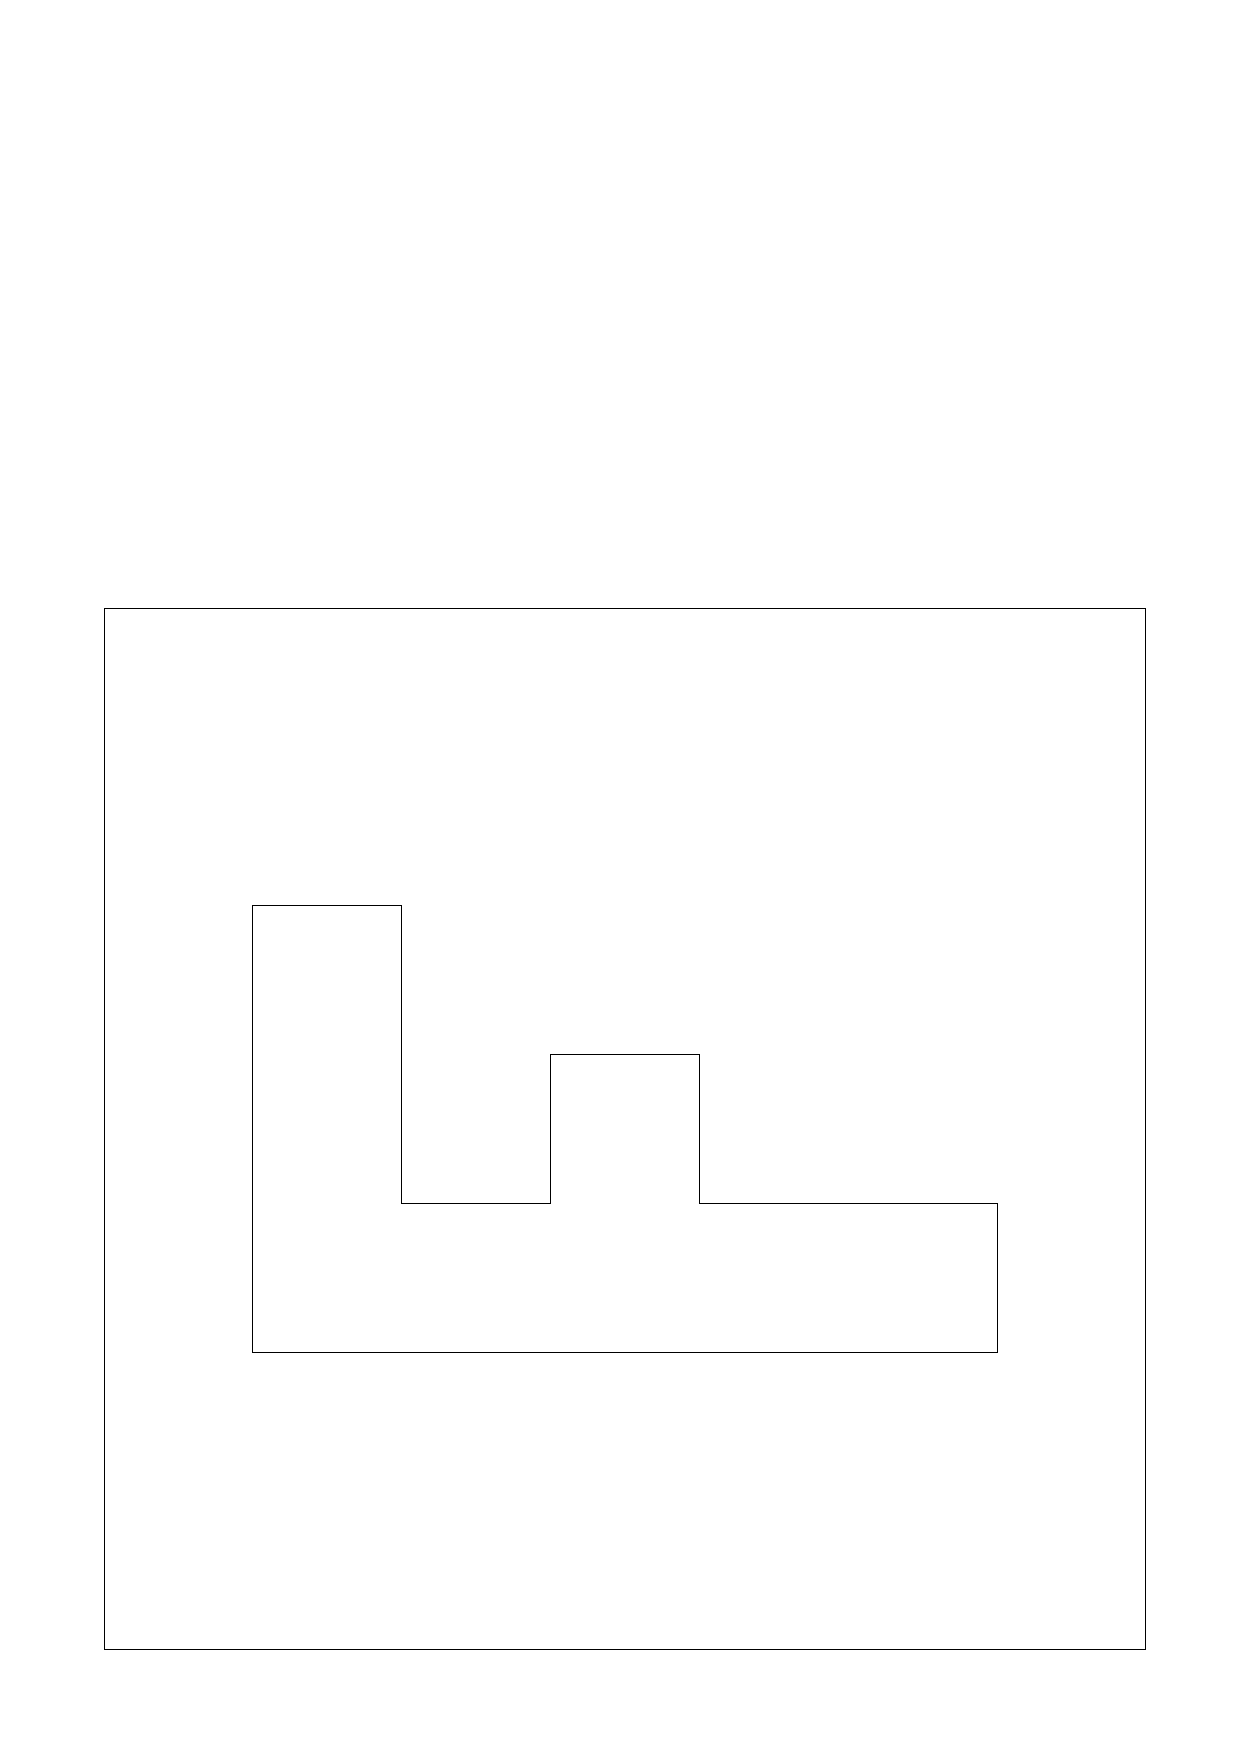
\includegraphics[width=0.4\textwidth]{./figs/basic/rot_f}
            \caption{\texttt{rot(f)}}
            \label{fig:rot_f}
        \end{figure}
    \end{frame}

    \begin{frame}{Flip}
        Voltea una imagen a lo largo de su eje central

        \begin{figure}
            \centering
            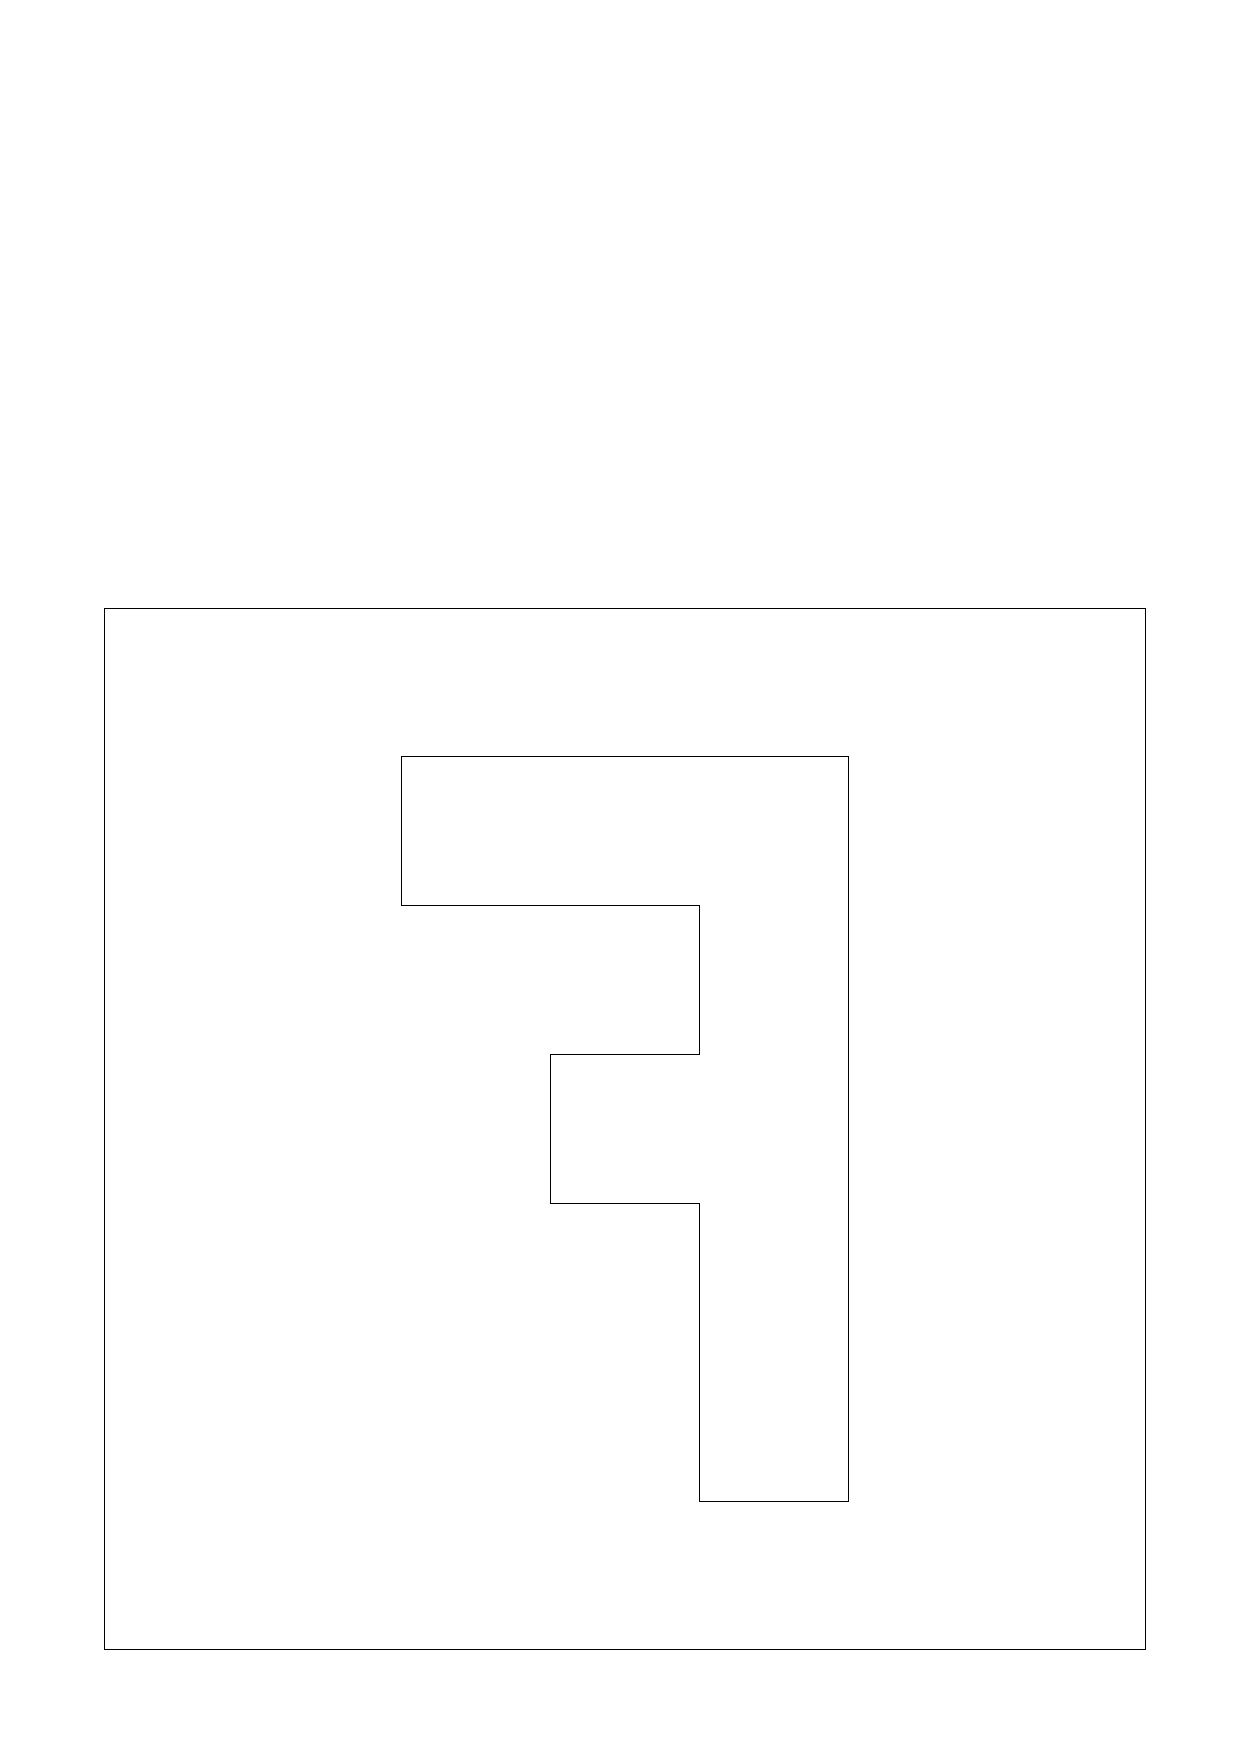
\includegraphics[width=0.4\textwidth]{./figs/basic/flip_f}
            \caption{\texttt{flip(f)}}
            \label{fig:flip_f}
        \end{figure}
    \end{frame}

    \begin{frame}{Rotacion y Flip}
        Aplica \texttt{flip(f)} a la imagen y seguidamente \texttt{rot()}

        \begin{figure}
            \centering
            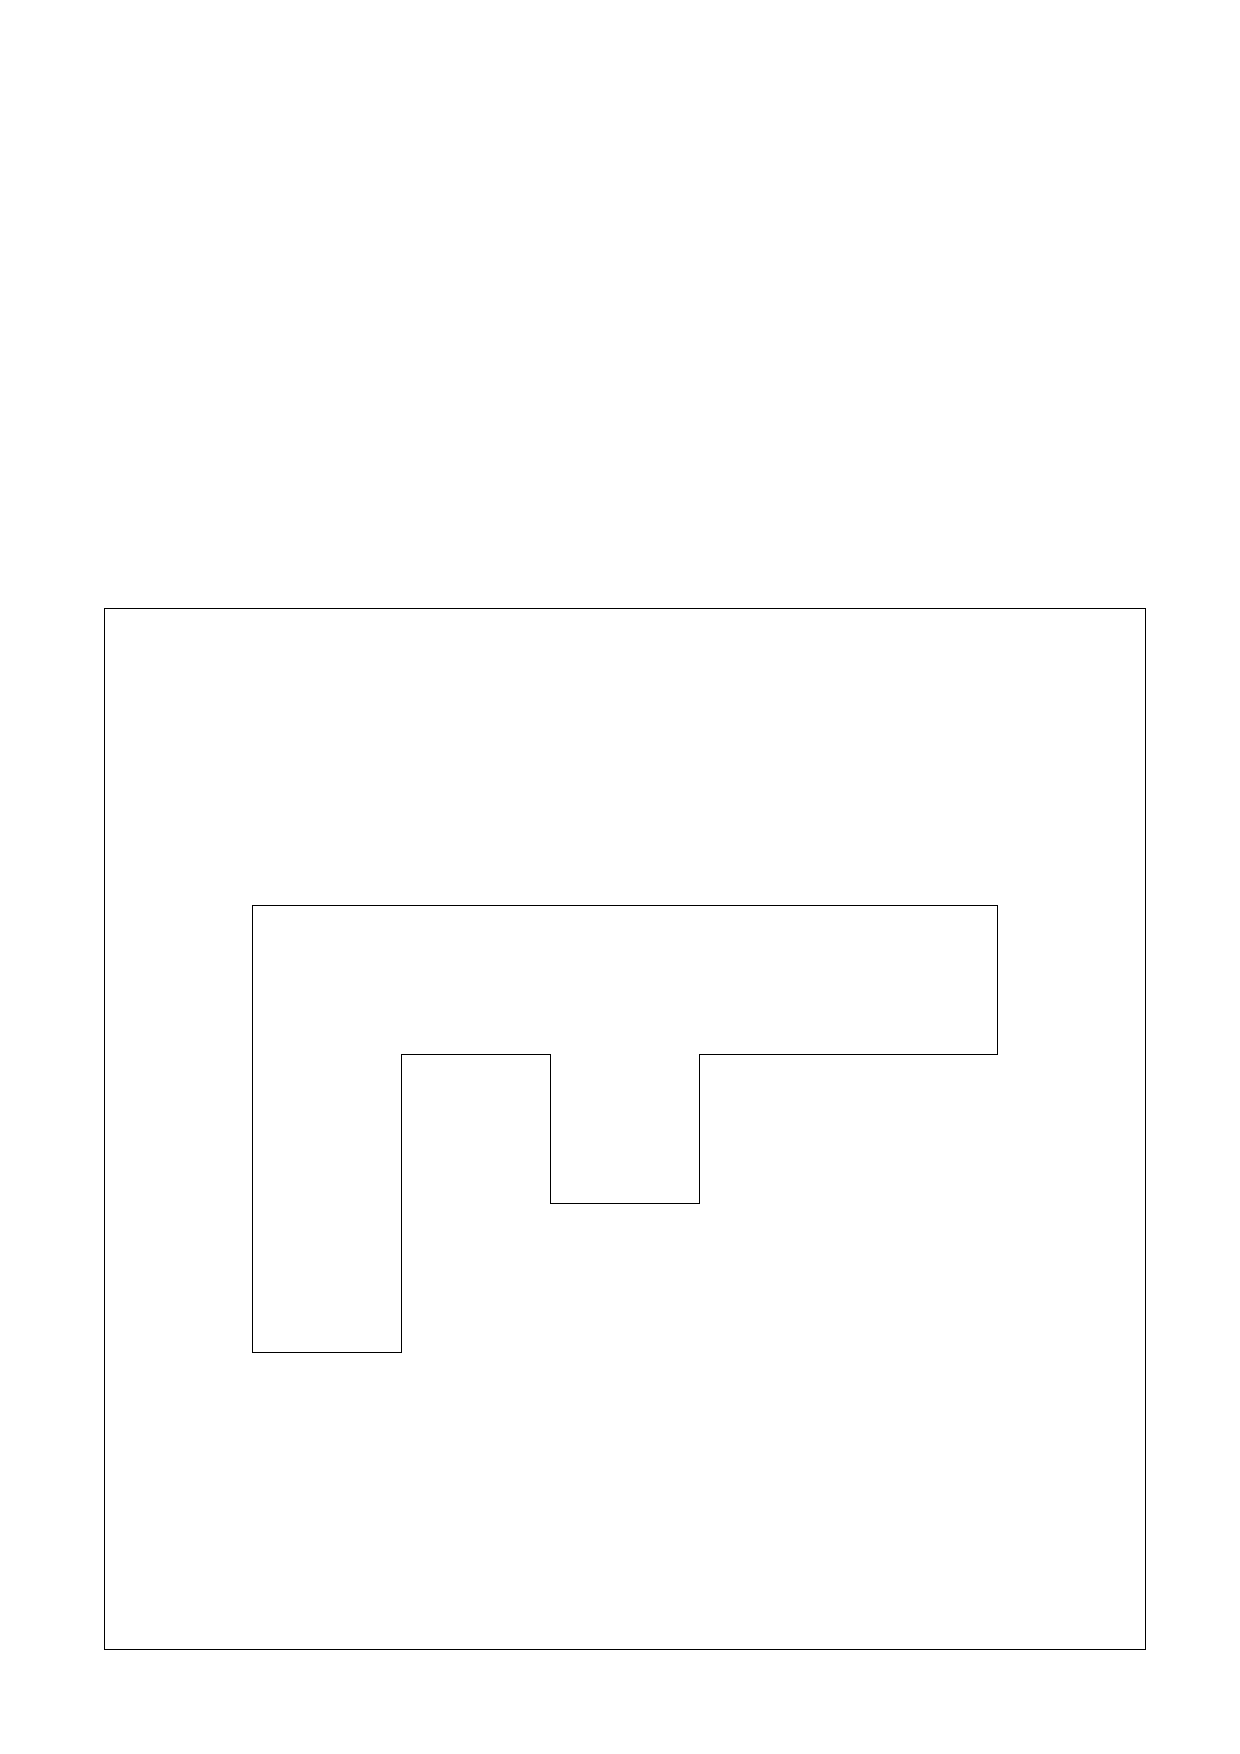
\includegraphics[width=0.4\textwidth]{./figs/basic/rot_flip_f}
            \caption{\texttt{rot(flip(f))}}
            \label{fig:rot_flip_f}
        \end{figure}
    \end{frame}

    \begin{frame}{Rotacion 45$^{\circ}$}
        \begin{figure}
            \centering
            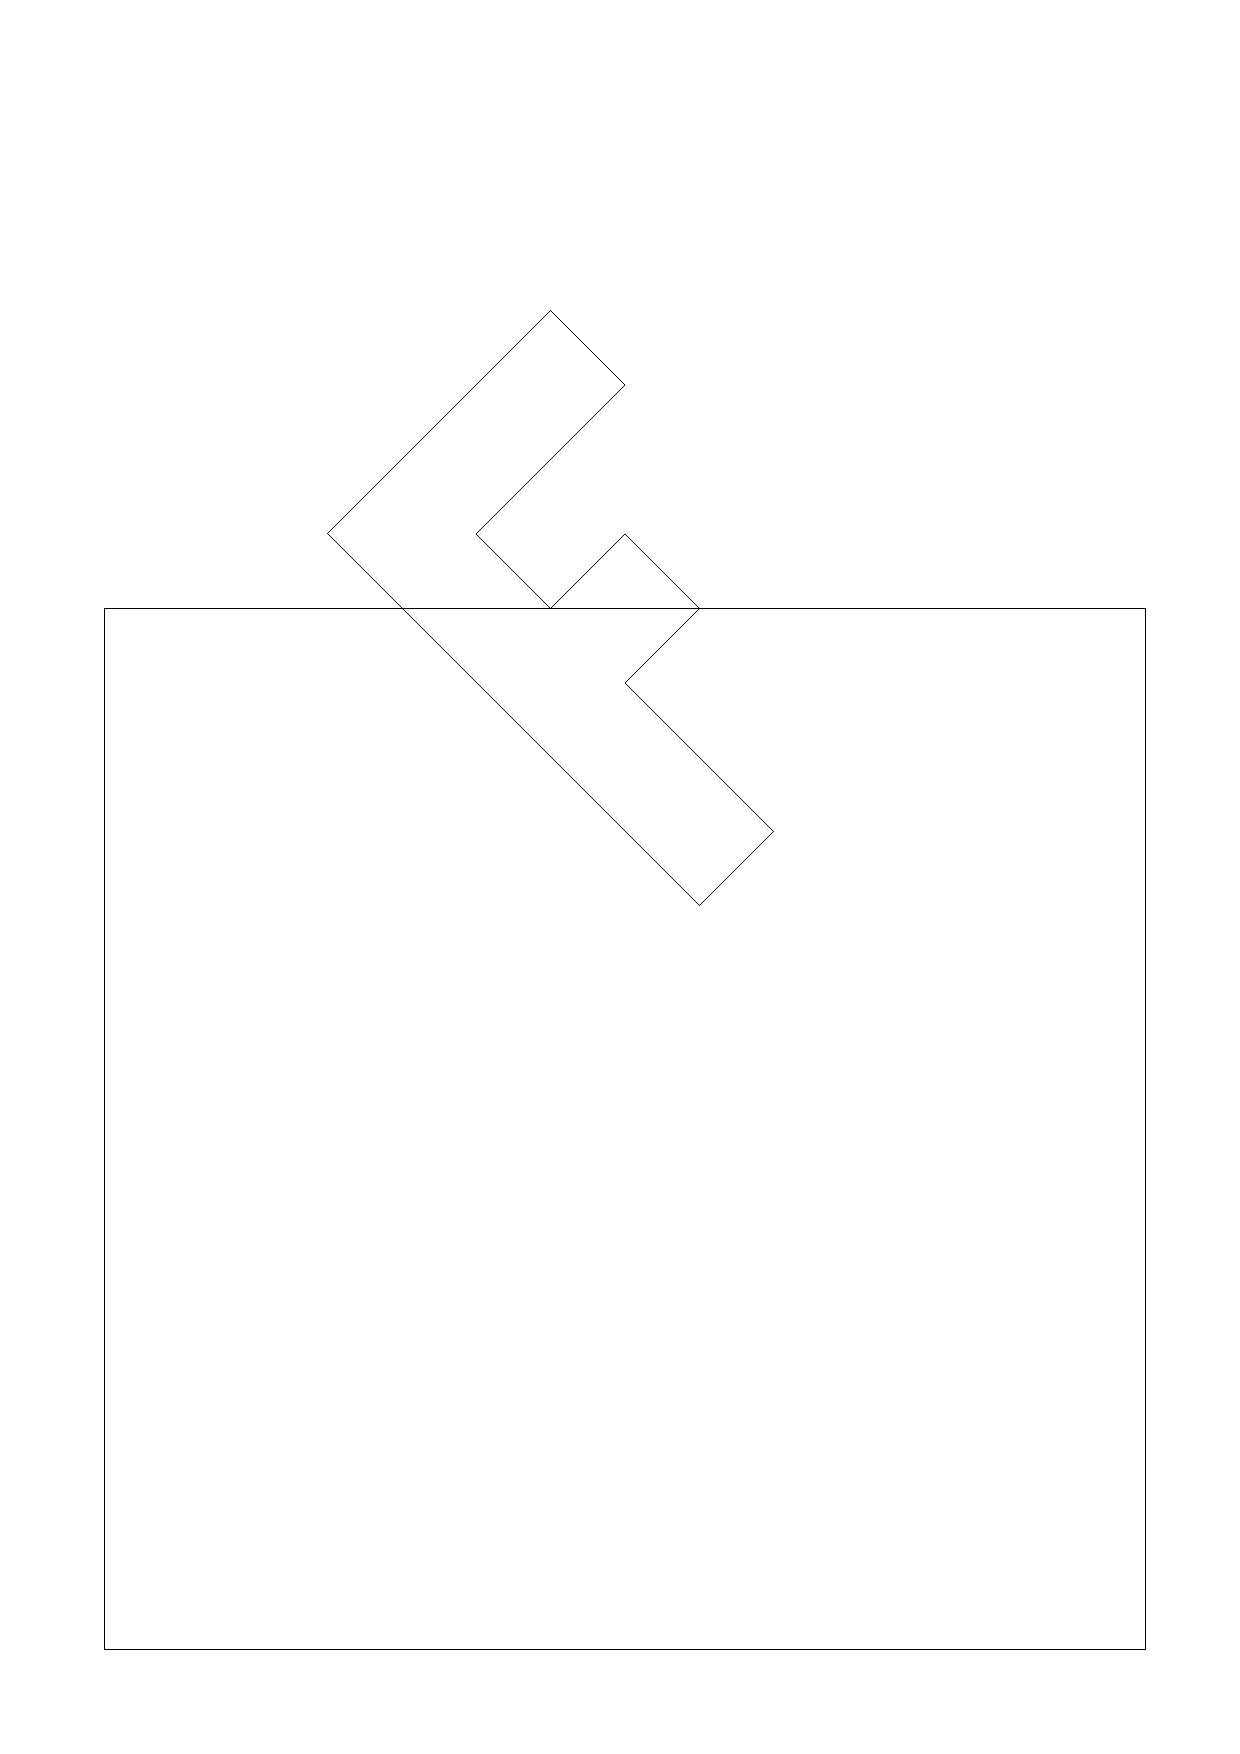
\includegraphics[width=0.4\textwidth]{./figs/basic/rot45}
            \caption{\texttt{rot45(f)}}
            \label{fig:rot45}
        \end{figure}
    \end{frame}

    \begin{frame}{Encima}
        \begin{figure}
            \centering
            
\includegraphics[width=0.4\textwidth]{./figs/basic/above_f}
            \caption{\texttt{above(f, f)}}
            \label{fig:above}
        \end{figure}
    \end{frame}

    \begin{frame}{Al lado}
        \begin{figure}
            \centering
            
\includegraphics[width=0.4\textwidth]{./figs/basic/beside_f}
            \caption{\texttt{beside(f, f)}}
            \label{fig:beside}
        \end{figure}
    \end{frame}

    \begin{frame}{Combinacion above/beside}
        \begin{figure}
            \centering
            
\includegraphics[width=0.4\textwidth]{./figs/basic/above_beside_f}
            \caption{\texttt{above(beside(f, f) f)}}
            \label{fig:above_beside_f}
        \end{figure}
    \end{frame}

    \begin{frame}{Superposicion}
        \begin{figure}
            \centering
            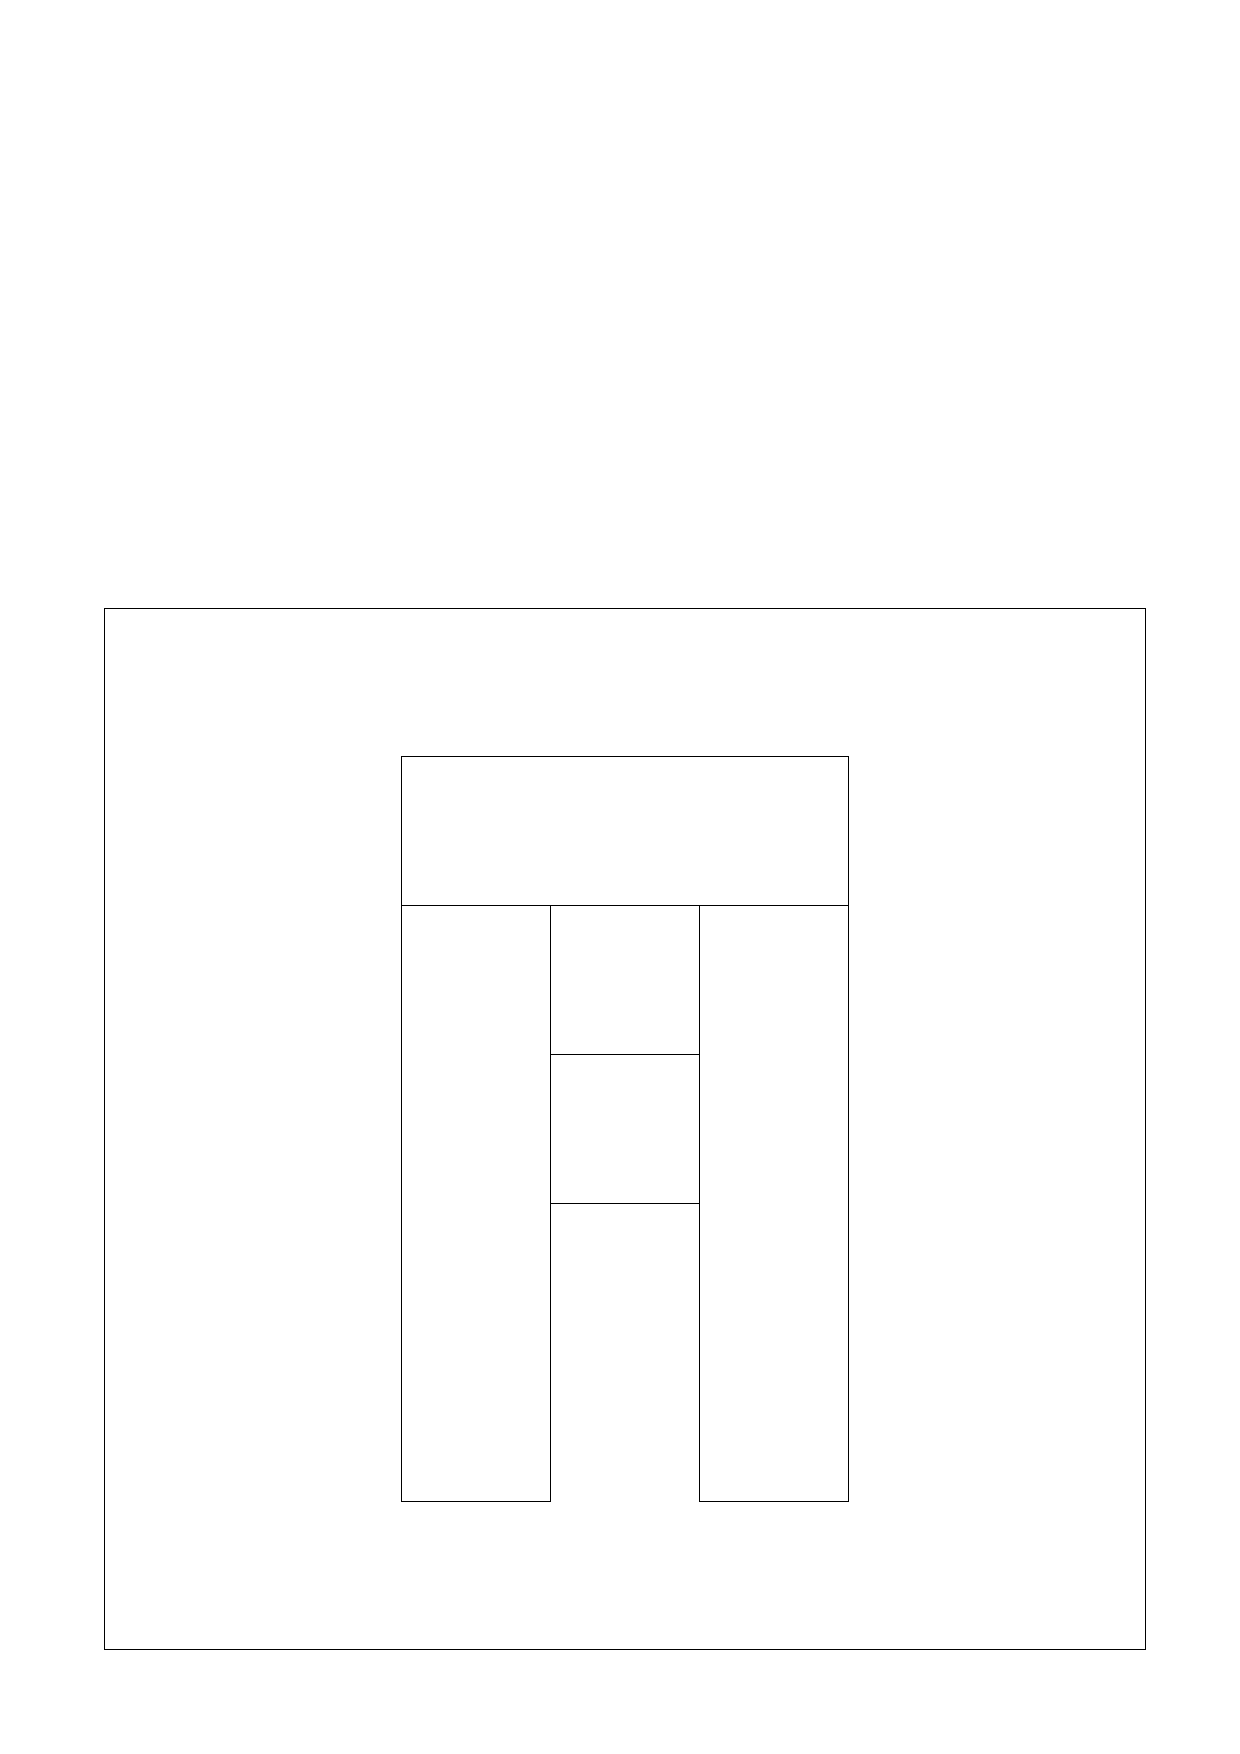
\includegraphics[width=0.4\textwidth]{./figs/basic/over}
            \caption{\texttt{over(f, flip(f))}}
            \label{fig:over_f}
        \end{figure}
    \end{frame}

	\section{Laws}
	
	\begin{frame}{Laws}
		\begin{equation*}
			rot(rot(rot(rot(p)))) = p
		\end{equation*}
	\end{frame}
		
	\begin{frame}{Laws}
		\begin{equation*}
			rot(above(p, q)) = beside(rot(p), rot(q))
		\end{equation*}

		\begin{equation*}
			rot(beside(p, q)) = above(rot(q), rot(p))
		\end{equation*}

		\begin{equation*}
			flip(beside(p, q)) = beside(flip(q), flip(p))
		\end{equation*}
	\end{frame}

	\section{Implementation}

	\begin{frame}{Implementation}
		\begin{equation*}
		over(p, q)(a, b, c) = p(a, b, c) \cup q(a, b, c)
		\end{equation*}

		\begin{equation*}
		blank(a, b, c) = \text{{}}
		\end{equation*}

		\begin{equation*}
		beside(p, q)(a, b, c) = p(a, \frac{b}{2}, c) \cup q(a + \frac{b}{2}, \frac{b}{2}, c)
		\end{equation*}

		\begin{equation*}
		above(p, q)(a, b, c) = p(a, b, \frac{c}{2}) \cup q (a + \frac{c}{2}, b, \frac{c}{2})
		\end{equation*}
	\end{frame}
		
	\begin{frame}{Implementation}
		\begin{equation*}
		rot(p)(a, b, c) = p(a + b, c, -b)
		\end{equation*}

		\begin{equation*}
		flip(p)(a, b, c) = p(a + b, -b, c)
		\end{equation*}
		
		\begin{equation*}
		rot45(p)(a, b, c) = p(a + \frac{b + c}{2}, \frac{b + c}{2}, \frac{c - b}{2})
		\end{equation*}
	\end{frame}

	\begin{frame}[standout]
		Demo :)
	\end{frame}

	\begin{frame}{Posibles mejoras}
		\begin{itemize}
			\item Proveer salida en \url{https://developer.mozilla.org/en/docs/Web/SVG/Tutorial/Paths}{SVG Path}
			\item Crear un API para interactuar, desde el front-end crear algo similar a Snap o Scratch
			\item Profundizar en el paper de los franceses
		\end{itemize}
	\end{frame}

	\begin{frame}[standout]
		Gracias!
	\end{frame}

\end{document}
